\chapter{Logic-Based Classification}
\label{logic-based-classification}

The concept bottleneck pipeline \cite{RefWorks:RefID:35-koh2020concept} uses human-explainable high-level concepts in the intermediate layer to find reasons for choosing a particular label.
These concepts should help a human understand why a prediction happened.
However, just because concepts are predicted does not mean they are indeed used in the final prediction.

For example, a network may learn a pattern which predicts a label \emph{out}, if some concept has a value greater than 0.2.
Yet, the model would not show such a concept to the user as relevant for the final prediction.
As we have done in the Chapter \ref{concept-bottleneck-pipeline}, showcasing the concepts after the attention layer would present the concepts more relevant for the final prediction.
Still, the attention layer presents the weight each concept has in the final prediction, but not the logic the MLP uses to choose the final label.

A fully interpretable method for predicting the final label would provide a clear link between the concepts and the outcomes.
In addition, models from concepts to the label can be validated and should, in an ideal case, follow the same logic as humans.

This chapter presents Prob-FF-NSL, an ILP-based classification method to improve the concept bottleneck model interpretability. 
The method works with probabilistic facts, allowing it to be incorporated into a concept bottleneck pipeline (Chapter \ref{concept-bottleneck-pipeline}).
Nevertheless, it is not limited to text concepts; it applies to any interpretable probabilistic NN output. 
% INSERT ref to evaluation
In section \ref{sudoku-grid-learning}, we evaluate it with outcomes of an image classification task.
The ILP system utilised for this task is FastLAS \cite{RefWorks:RefID:19-law2020fastlas:}, a scalable system that incorporates criteria for domain-specific optimisation.

\section{Changes to the Concept Bottleneck Architecture}
\label{change-to-the-concept-bottleneck-architecture}

An introduction of the rule learning component would result in the change in the concept bottleneck architecture shown in the figure \ref{logic-based-concept-bottleneck}.
\begin{figure}[h]
\caption{A flowchart to select an outcome of a multi-class classification problem.}
\vspace{10pt}
\centering
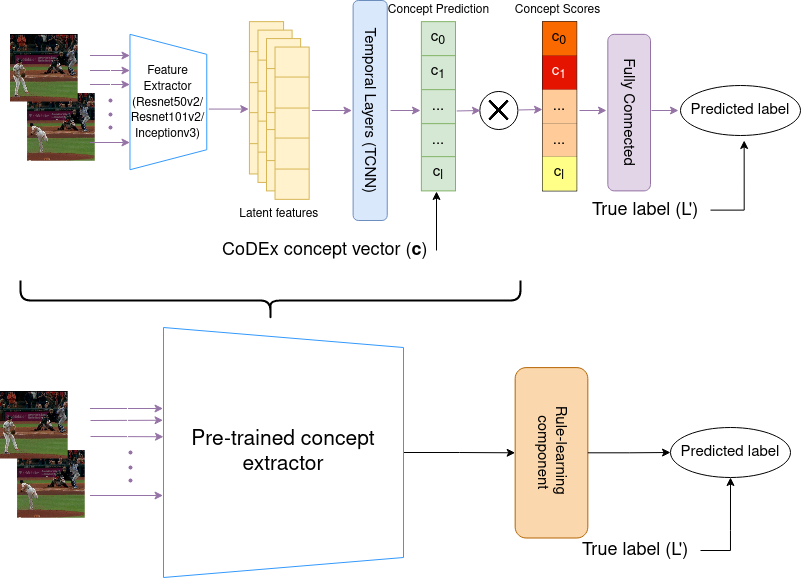
\includegraphics[width=\textwidth]{logic-based-classification/logic-based-classification-architecture.png}
\label{logic-based-concept-bottleneck}
\end{figure}

Training a concept bottleneck pipeline then turns into a 3-step process:
\begin{enumerate}
    \item Train a model in the same manner as in the Chapter \ref{concept-bottleneck-pipeline}, by minimising the loss CoDEx concept vector and final label prediction loss.
    \item Generate examples for the rule-learning component using the concepts predicted by the model from the step 1). Each example needs to take into account the probabilities of all concepts.
    \item Train the rule-learning component.
\end{enumerate}

At run-time, predict the concepts using the model trained in step 1 before applying the rules learned in step 3 to obtain the final prediction.

The ASP paradigm does not support any notion of probability; an atom can either be in or out of an answer set. 
So, to force the learner to treat less likely cases differently, we carefully choose the FastLAS example penalties, similar to Cunnington et al. \cite{RefWorks:RefID:71-cunnington2021ff-nsl:}.
However, we aim to use those penalties to find the most likely solution.

\section{Choosing FastLAS Parameter Values}
\label{choosing-fastlas-parameter-values}

% INSERT reference to background section decomposable
FastLAS can find an optimal solution with respect to a scoring function of kind ($\curly{S} + \curly{S}_{pen}$), where $\curly{S}$ is a decomposable scoring function (\ref{fastlas-background}) and $\curly{S}_{pen}$ is a sum of all uncovered example penalties.

In this section, we attempt to find the appropriate scoring function $\curly{S}$ and values for penalties such that the final solution is highly likely given the learning task tuple $T = \langle B, M, E_{prob} \rangle$. 

\subsection{Used Notation}

Let our set of examples $E_{prob}$ be $\{(\vec{x}_e, y_e)\}_{e=1}^{E} \in \curly{E}$ with $E$ examples. 
An example $(\vec{x}_e, y_e)$ consist of a vector of concept probabilities $\vec{x}_e = (x_{ec})_{c=1}^C$ and a label $y_e \in \curly{L}$ assigned to the example $e$ from the set of possible labels $\curly{L}$.
The symbol $x_{ec}$ denotes a priori probability that concept $c$ takes truth value (=1) in example $e$.
Moreover, $C$ is the number of extracted concepts for a given problem. \\
We can represent examples as a matrix of concept probabilities.  
The examples can be represented as an input matrix of concept probabilities $\vec{X} = (\vec{x}_e^T)_{e=1}^E$ and an output vector of target labels $\vec{y} = (y_e)_{e=1}^E$.

Let $\curly{H}$ be the set of all possible hypotheses. The term $p(y_e|H, \vec{x}_{e})$ represents the probability that the example $e$ is covered, for any hypothesis $H \in \curly{H}$,


We introduce notation for grounded examples, as answer sets can only contain grounded atoms.
A grounded example $(\vec{z}_e, y_e)$ is an example where each concept $c$ in an example $e$ is assigned a truth value $z_{ec} \in \{0,1\}$ (integer form). 
The term $\vec{z}_e = (z_{ec})_{c=1}^C \in \curly{Z}_e$  is a binary vector representing the ground assignment. 

\subsection{Determining Optimal Example Penalties}

We want to choose the example penalties such that the FastLAS output hypothesis $H$ is the maximum-likelihood hypothesis $H_{\text{ML}}$, i.e. the output hypothesis should satisfy the following equation:
\begin{align}
H_{\text{ML}} = \arg\max_{H}
p(\vec{y}|H, \vec{X})
\end{align}

Making an assumption that given a model and concept probabilities, the labels for any two examples are conditionally independent we can rewrite the term $p(\vec{y}|H, \vec{X})$ in the following manner:
\begin{align}
p(\vec{y}|H, \vec{X})
= \prod_{e} p(y_e|H, \vec{x}_e) \label{eq6.3}
\end{align}


As the $ln = log_e$ function is monotonically increasing in the range $(0, \infty)$ and as the above equation produces values in that range, it is equivalent to maximising the $ln$, resulting in the following optimisation target:
\begin{align}
H_{\text{ML}}
& = \arg\max_{H}
\ln p(\vec{y}|H, \vec{X}) \nonumber \\
& = \arg\max_{H}
\sum_{e} \ln p(y_e|H, \vec{x}_e) && \text{(by \ref{eq6.3})} \nonumber \\
& = \arg\min_{H}
-\sum_{e} \ln p(y_e|H, \vec{x}_e) && \text{(alternative objective)} \label{ex6.4}
\end{align}


% TODO: define Z
We can now calculate the probability that a label $y_e$, for example $e$, is covered by a hypothesis $H$ where we know the set of concept probabilities $\vec{x}_e$.
That probability is computed by considering all possible grounding that $\vec{x}_e$ induces.
It is given by:
\begin{align}
p(y_e|H, \vec{x}_e)
& = \sum_{\vec{z} \in \curly{Z}_e} p(y_e, \vec{z} | H, \vec{x}_e) && \text{(sum rule)} \nonumber \\
& = \sum_{\vec{z} \in \curly{Z}_e} p(y_e | \vec{z}, H, \vec{x}_e) p(\vec{z} | H, \vec{x}_e) && \text{(conditional probability)} \nonumber \\
& = \sum_{\vec{z} \in \curly{Z}_e} p(y_e | \vec{z}, H) p(\vec{z}| \vec{x}_e) && \text{(by independence)} \nonumber \\
& = \expct_{\vec{z} \sim p(\vec{z}| \vec{x}_e)}[p(y_e|\vec{z},H)] \label{ex6.5}
\end{align}

Considering the $\ln$ of the term above, we can use the Jensen's inequality to push it inside the expectation:
\begin{align}
\ln p(y_e|H, \vec{x}_e)
&= \ln \expct_{\vec{z} \sim p(\vec{z}| \vec{x}_e)}[p(y_e|\vec{z},H)] \nonumber \\
&\leq \expct_{\vec{z} \sim p(\vec{z}| \vec{x}_e)}[\ln  p(y_e|\vec{z},H)] 
\nonumber \\
\end{align}

We further assume that the bounds of Jensen's inequality are sufficiently tight, i.e. we assume that:
\begin{align}
\ln p(y_e|H, \vec{x}_e)
&\approx \expct_{\vec{z} \sim p(\vec{z}| \vec{x}_e)}[\ln  p(y_e|\vec{z},H)] \label{jensen-approx}
\end{align}

Now we can estimate the expectation by sampling $I$ ground examples for example $e$, where ground examples are $\vec{z}_{i} \sim p(\vec{z}| \vec{x}_e)$, then:
\begin{align}
\expct_{\vec{z} \sim p(\vec{z}| \vec{x}_e)}[\ln  p(y_e|\vec{z},H)]
\approx \frac{1}{I} \sum_{i=1}^{I} \ln  p(y_e|\vec{z}_i,H) \label{sampling-result}
\end{align}

For some hypothesis, $H\in \curly{H}$, a grounded example is or is not covered by $H$. We allow a label to be incorrect with some small error $\epsilon > 0$, resulting in the following probabilistic interpretation:
\begin{align}
p(y_e | \vec{z}, H) =
\begin{cases}
1 - \epsilon & \text{if } H, \vec{z} \models y_e \\
\epsilon & \text{otherwise}
\label{def-ground}
\end{cases}
\end{align}

Combining all the results presented, we can derive the following:
\begin{align}
H_{\text{ML}} 
& = \arg\max_{H}
p(\vec{y}|H, \vec{X}) \nonumber \\
& = \arg\min_{H} 
-\sum_e \ln \left( \expct_{\vec{z} \sim p(\vec{z}| \vec{x}_e)}[p(y_e|\vec{z},H)] \right ) 
&& \text{(by \ref{ex6.4} and \ref{ex6.5})} \nonumber \\
& \approx \arg\min_{H}
-\sum_e \expct_{\vec{z} \sim p(\vec{z}| \vec{x}_e)}[\ln \left[ p(y_e|\vec{z},H) \right ]]  
&& \text{(by \ref{jensen-approx})} \nonumber \\
& \approx \arg\min_{H}
\sum_e \frac{1}{I} \sum_{i=1}^I -\ln \left[ p(y_e|\vec{z},H) \right ]
&& \text{(by \ref{sampling-result})} \nonumber \\
& = \arg\min_{H} \sum_e \frac{1}{I} \sum_{i=1}^I  \left(-\ln  [p(y_e|\vec{z}_{ei},H)] + \ln (1-\epsilon) \right)
&& \text{(constant shift)} \nonumber \\
& = \arg\min_{H}
\sum_e \frac{1}{I} 
\left (
\sum_{H,\vec{x}_{ei}\models y_e} 0
+
\sum_{H,\vec{x}_{ei}\not\models y_e} (-\ln \epsilon + \ln (1 - \epsilon))
\right ) 
&& \text{(by \ref{def-ground})} \nonumber \\
& = \arg\min_{H}
\sum_e  
\sum_{H,\vec{x}_{ei}\not\models y_e} -\frac{1}{I}\ln \left ( \frac{\epsilon}{1 - \epsilon} \right ) \label{eq-final-no-int}
\end{align}


Optimising only for the $\curly{S}_{pen}$, FastLAS would return the following solution:
\begin{align}
H
& = \arg\min_{H}
\sum_e  
\sum_{H,\vec{x}_{ei}\not\models y_e} e_{pen}
\end{align}

Hence, by setting the penalty for each example to $-\frac{1}{I} \ln \left ( \frac{\epsilon}{1 - \epsilon} \right )$ and prior (hypothesis) penalties to 0, FastLAS would return a solution close to the maximum likelihood for all examples.

\subsubsection{Integer penalties}
\label{integer-penalties}

FastLAS does not support any floating point number calculations, including penalty values, making the expression derived above unusable.

But, we can overcome this issue.
Let us consider a large value $K \in \reals^+$, and then round $K$ multiplied by each term in the sum to the nearest integer. Because for large enough $K$:
\begin{align}
    Kt \approx round(Kt) \label{rounding}
\end{align}

In addition, minimising any $t \in \reals^+$ is equivalent to minimising $K t$ for any $K \in \reals^+$.
So, the function we wish to minimise becomes: 
\begin{align}
H_{\text{ML}}
& = \arg\min_{H}
\sum_e  
\sum_{H,\vec{x}_{ei}\not\models y_e} -\frac{1}{I}\ln \left ( \frac{\epsilon}{1 - \epsilon} \right ) 
&& \text{(\ref{eq-final-no-int})} \nonumber \\
& = \arg\min_{H}
K \sum_e  
\sum_{H,\vec{x}_{ei}\not\models y_e} -\frac{1}{I}\ln \left ( \frac{\epsilon}{1 - \epsilon} \right ) 
&& \text{(scaling $t \in \reals^+$ by $K \in \reals^+$)} \nonumber \\
& = \arg\min_{H}
\sum_e  
\sum_{H,\vec{x}_{ei}\not\models y_e} -\frac{K}{I}\ln \left ( \frac{\epsilon}{1 - \epsilon} \right ) \nonumber \\ 
& = \arg\min_{H}
\sum_e  
\sum_{H,\vec{x}_{ei}\not\models y_e} \text{round} \left ( -\frac{K}{I}\ln \left ( \frac{\epsilon}{1 - \epsilon} \right ) \right )
&& \text{(by \ref{rounding})}
\end{align}

Therefore, after choosing some large $K > 0$, we assign the non-coverage penalty of $\text{round} \left ( -\frac{K}{I} \ln \left ( \frac{\epsilon}{1 - \epsilon} \right ) \right )$ to each example.

\subsection{Incorporating a Prior over the Hypothesis Space}

Now, we can extend the approach done in the previous section by considering a prior over hypothesis space ($p(H)$) too.
The extension would give a plausibility value to each potential $H$ before evaluating its fitness on the examples. 
We can combine this with the likelihood function to give a posterior probability for the data and hypothesis, namely:
\begin{align}
p(\vec{y}, H|\vec{X})
& = p(\vec{y}|H, \vec{X})p(H)
\end{align}

We can log this to get:
\begin{align}
\ln p(\vec{y}, H|\vec{X})
& = \ln p(\vec{y}|H, \vec{X}) + \ln p(H)
\end{align}

% INSERT reference to MAP estimate paper NOREF
Maximising the above equation leads to what we would call the maximum posterior estimate for $H$, or maximum a posteriori (MAP) estimate:
\begin{align}
H_{\text{MAP}}
& = \arg\max_{H} \ln p(\vec{y}|H, \vec{X}) + \ln p(H) 
\end{align}

% As with the maximum likelihood approach we can maximise the rescaled expression using $K \in \reals^+$ giving:
% \begin{align}
% h_{\text{MAP}}
% & = \arg\max_{h} \left(K\ln p(\vec{y}|h, \vec{X}) + K\ln p(h) \right)
% \end{align}

% Or we can see this as minimising a negative log-loss:
% \begin{align}
% h_{\text{MAP}}
% & = \arg\min_{h} \left(-K\ln p(\vec{y}|h, \vec{X}) - K\ln p(h) \right)
% \end{align}

% Note the important point here is that the scale of the penalties on the prior must match the scale of penalties on the examples.

\subsubsection{Choosing a Meaningful Prior over the Hypothesis Space}

There are several ways to place a prior on hypothesis space. 
The default ILASP \cite{RefWorks:RefID:18-law2020ilasp} and the usual FastLAS approach assign smaller penalties, i.e., higher prior probabilities, to shorter clauses.
% INSERT online symbolic learning of policies for explainable security DONE
Some problems benefited from assigning lower penalties to "ideal length" rules, such as Drozdov et al. \cite{RefWorks:RefID:67-drozdov2021online}.

We have opted for a slightly different approach that we can incorporate well into the theory presented thus far. \\
Starting with a set of potential rules $\curly{R}$, let $q_r$ be an independent probability that $r$ is included in $H$ (written $r \in H$) for every potential rule $r \in \curly{R}$. Then the prior probability can be written as:
\begin{align}
p(H) = \left(\prod_{r \in H} q_r\right)\left(\prod_{r \in \curly{R}\setminus H} (1-q_r)\right)
\end{align}

We can log this for convenience:
\begin{align}
\ln p(H) = \sum_{r \in H} \ln q_r + \sum_{r \in \curly{R}\setminus H} \ln(1-q_r) \label{log-prior-rule}
\end{align}


For a fixed reference hypothesis such as $H_0 = \emptyset$, maximising the posterior is equivalent to maximising the posterior divided by the prior, resulting in:
\begin{align}
H_{\text{MAP}}
& = \arg\max_{H} p(\vec{y}|H, \vec{X}) p(H)  \nonumber \\
& = \arg\max_{H} \left(\frac{ p(\vec{y}|H, \vec{X}) p(H)}{p(H_0)}\right)  \nonumber \\
& = \arg\min_{H} \left( -K\ln p(\vec{y}|H, \vec{X}) - K \ln \frac{p(H)}{p(H_0)}\right) \label{h-map-final}
\end{align}
The above equation holds for some $K > 0$, added to deal with FastLAS inability to work with non-integers as in \ref{integer-penalties}.

The ratio of the overall change in prior for any hypothesis $H \in \curly{H}$ from the empty hypothesis $H_0 = \emptyset$ can then be calculated using \ref{log-prior-rule} as follows:
\begin{align}
\ln \left(\frac{p(H)}{p(H_0)}\right) 
& = \sum_{r \in H} \ln q_r + \sum_{r \in \curly{R}\setminus H} \ln(1-q_r) \nonumber
- \sum_{r \in \emptyset} \ln q_r - \sum_{r \in \curly{R}} \ln(1-q_r) \\
& = \sum_{r \in H} \left(\ln q_r - \ln(1-q_r) \right)
\end{align}

As FastLAS finds an optimal solution with respect to the scoring function ($\curly{S}_{pen} + \curly{S}$), it can satisfy the equation \ref{h-map-final} if we choose the examples penalties as in \ref{integer-penalties} and the following $\curly{S}$:
\begin{align}
    \curly{S}(H, T) =  -K \sum_{r \in H} \left(\ln q_r - \ln(1-q_r) \right)
\end{align}
By inspection, we see that the decomposition of the function $\curly{S}$ is given by:
\begin{align}
    \curly{S}^{rule}(r, T) = -K (\ln q_r - \ln(1-q_r))
\end{align}


Finally, we need to choose appropriate values probabilities $q_c$. \\
Imagine that we have a rule of length $l$, we would expect to find $m_l$ clauses of length $l$ in a specific hypothesis, and there are $n_l$ clauses of length $l$ in the set of all possible rules $\curly{R}$. 
This setup suggests a value for $q_{r_l} = \frac{m_l}{n_l}$, resulting in the following change to the $\curly{S}^{rule}$:
\begin{align}
\curly{S}^{rule}(r, T) 
& = -K (\ln q_r - \ln(1-q_r)) \nonumber \\
& = -K \left (\ln \frac{m_l}{n_l} - \ln \frac{n_l - m_l}{n_l} \right) \nonumber \\
& = K \left (\ln (n_l - m_l) - \ln m_l  \right)
\end{align}

\section{Implementation}

% TODO: merge binary classification and multi-label classification into one subsection
\subsection{Encoding Binary Classification Task}
\label{encoding-binary-classification-task}

To encode a solution to a binary classification problem using ASP, we can do the following:
\begin{itemize}
    \item Write rules such as \verb+label1 :- ...+  for one of the labels.
    \item Add the rule of the form \verb+label2 :- not label1+.
\end{itemize}

% TODO: remove the itemise and encode is as a piece of text
With this approach, we are guaranteed to have precisely one label in each answer set of the task.
We always want exactly one answer set as a solution, as we always want just one outcome.
To prevent that possibility from occurring, the following types of ASP rules are not used:
\begin{itemize}
    \item Choice rules --- Choice rules give rise to multiple answer sets, which we do not want.
    \item "Not-chain" --- Combination of normal rules which can only be satisfied by multiple answer sets, such as \verb+{p :- not q. q :- not p.}+. The program satisfying the "non-chain" requirement is stratified. This means that its rules can be split into disjoint multiple strata $P = P_0 \cup P_1 \cup ... \cup P_n$ where each strata $P_i$ can only have negations of atoms defined in $P_0 \cup ... \cup P_{i-1}$.
    \item Constraints --- Constraints are used to eliminate an answer set from occurring. If we were to remove the single occurring answer set, we would not get a solution.
\end{itemize}

An alternative to this encoding which would return a solution with the highest score is also possible. However, it is not nearly as interpretable.

\begin{example}
\label{sudoku-binary-example}
Encoding the sudoku learning task:

% INSERT reference evaluation
The sudoku 4x4 learning task (\ref{sudoku-grid-learning}) should deduce whether a grid is or is not valid.

1. \textit{Construct the background knowledge:} \\
The background knowledge for sudoku could contain the following rules that specify which row/column/block a cell belongs to.
\begin{verbatim}
num(1..4).
col(1..4).
row(1..4).
block(1..4).
% value(C, N) represents that number N is written in cell C
cell(C) :- value(C, _).

col((X, Y), Y) :- row(X), col(Y).
row((X, Y), X) :- row(X), col(Y).
block((X, Y), 1) :- row(X), col(Y), X <= 2, Y <= 2.
block((X, Y), 2) :- row(X), col(Y), X <= 2, Y > 2.
block((X, Y), 3) :- row(X), col(Y), X > 2, Y <= 2.
block((X, Y), 4) :- row(X), col(Y), X > 2, Y > 2.

neq_cell(C1, C2) :- cell(C1), cell(C2), C1 != C2.
\end{verbatim}

2. \textit{Account for the alternative label:} \\
We add the following rule to the background knowledge:
\begin{verbatim}
selected(valid) :- not selected(invalid). 
\end{verbatim}

3. \textit{Construct the language bias:} \\
We chose that we wish to learn what makes a cell invalid in this example, resulting in the following language bias:
\begin{verbatim}
#modeh(selected(invalid)).

#modeb(row(var(cell), var(row))).
#modeb(col(var(cell), var(col))).
#modeb(block(var(cell), var(block))).
#modeb(neq_cell(var(cell), var(cell))).
#modeb(value(var(cell), var(num))).

#maxv(4).
\end{verbatim}

4. \textit{Add examples and prior penalty definitions:}
% INSERT refernce to example definition and prior penalty definition
We will discuss this step in the example \ref{sudoku4x4-examples-prior}.
\end{example}

\subsection{Encoding Multi-label Classification Task}

The multi-label classification outcome is decided using the flowchart in \ref{flowchart-multi-label-classification}, where the \verb_conds(label(x))_ predicate is true when conditions for a particular label are satisfied.

\begin{figure}[h]
\caption{A flowchart to select an outcome of a multi-label classification problem.}
\vspace{10pt}
\centering
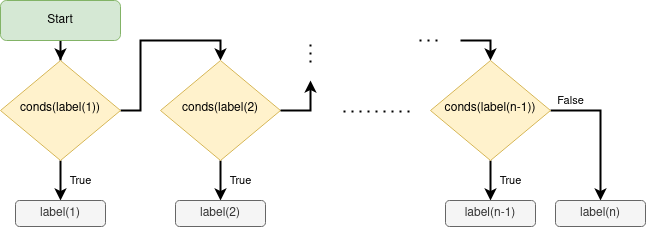
\includegraphics[width=\textwidth]{logic-based-classification/multi-label-selection.png}
\label{flowchart-multi-label-classification}
\end{figure}

We chose this flowchart structure to aid interpretability because FastLAS learns the following set of rules:
\begin{verbatim}
conds(label(1)) :- ...
conds(label(1)) :- ...
...
conds(label(n-1)) :- ...
conds(label(n-1)) :- ...
\end{verbatim}
So, a human can easily determine the outcome by going through the rules from top to bottom and selecting a label matching the first satisfied rule.
Learning these types of rules is encoded in FastLAS with the following syntax:
\begin{verbatim}
#modeh(conds(const(learnable_label))).

... all the modeb declarations ...

% Avoid constraints
#bias("
:- constraint.
").
\end{verbatim}

Furthermore, to make the learner use the logic presented in the flowchart, we need to encode the following: 
\begin{enumerate}
    \item The position of a label in the flowchart chain.
    \item Selection of the highest priority label whose conditions are satisfied.
    \item Selection of the lowest priority label when no conditions are satisfied.
\end{enumerate}
The enumerated criteria result in the following ASP encoding added to the background of a learning task:
\begin{lstlisting}
% Encoding 1 with label(name, position) (lower=better)
label(l1, 0).
label(l2, 1).
...
label(ln, n-1).

% Definitions of types for FastLAS
label(L) :- label(L, _).
learnable_label(L) :- exists_lower_priority(L, _).


% Encoding 2: Select the highest priority label whose conditions are satisfied
selected(L) :- label(L, P), conds(L), 
                 not higher_priority_selection(L, P).
higher_priority_selection(L, P) :- label(L, P), label(L2, P2), 
                                       P2 < P, selected(L2).

% Encoding 3: Select default label if no higher priority selection is made
selected(L) :- label(L, P), not higher_priority_selection(L, P), 
                 not exists_lower_priority(L, P).
exists_lower_priority(L, P) :- label(L, P), label(L2, P2), P2 > P.
\end{lstlisting}

Notice that the presented encoding also produces exactly one answer set, the same as the encoding for the binary classification.

\begin{example}
Encoding the multi-class sudoku 4x4 learning task:

% INSERT reference evaluation
Consider an extension of the binary sudoku 4x4 task in the example \ref{sudoku-binary-example}, which introduces an additional label \verb_conflict_. 
That label should be true only when an example contains two digits written to the same cell.
The following steps are needed to solve the task using the presented multi-label classification encoding:

1. \textit{Construct the background knowledge:} \\
The background is the same as for the example \ref{sudoku-binary-example}.

2. \textit{Add the multi-label selection encoding to the background:} \\
We add the following rules to the background knowledge:
\begin{lstlisting}
% Encoding 1 with label(name, position) (lower=better)
label(conflict, 0).
label(invalid, 1).
label(valid, 2).

% Definitions of types for FastLAS
label(L) :- label(L, _).
learnable_label(L) :- exists_lower_priority(L, _).


% Encoding 2: Select the highest priority label whose conditions are satisfied
selected(L) :- label(L, P), conds(L), 
                 not higher_priority_selection(L, P).
higher_priority_selection(L, P) :- label(L, P), label(L2, P2), 
                                       P2 < P, selected(L2).

% Encoding 3: Select default label if no higher priority selection is made
selected(L) :- label(L, P), not higher_priority_selection(L, P), 
                 not exists_lower_priority(L, P).
exists_lower_priority(L, P) :- label(L, P), label(L2, P2), P2 > P.
\end{lstlisting}

2. \textit{Construct the language bias:} \\
We chose that we wish to learn what makes a cell invalid in this example, resulting in the following language bias:
\begin{verbatim}
#modeh(conds(const(learnable_label))).

#modeb(row(var(cell), var(row))).
#modeb(col(var(cell), var(col))).
#modeb(block(var(cell), var(block))).
#modeb(neq_cell(var(cell), var(cell))).
#modeb(value(var(cell), var(num))).

#maxv(4).
\end{verbatim}

4. \textit{Add examples and prior penalty definitions:}
% INSERT refernce to example definition and prior penalty definition
We will discuss this step in the example \ref{sudoku4x4-examples-prior}.
\end{example}


\subsection{Creating the Example File}

The example file incorporates the theory presented in \ref{choosing-fastlas-parameter-values}.
Recall from \ref{ilasp-background} that the FastLAS task allows defining positive and negative examples.
Positive examples are bravely entailed, i.e. the final solution should be extended by at least one answer set.
On the other hand, the negative examples are cautiously entailed, so the final solution must not be extended by any answer set.
Because of our classification encodings, the learned hypothesis can only ever return one answer set, making the positive examples sufficient to encode any task.

To account for FastLAS's inability to deal with probabilistic atoms, we need to sample $I$ examples, each of the form:
\begin{lstlisting}
#pos(example_id@$\text{round} \left ( -\frac{K}{I} \ln \left ( \frac{\epsilon}{1 - \epsilon} \right ) \right )$,
{selected(true_label)},
{selected(incorrect_label) for each incorrect_label}, 
{... context atoms derived from the raw example ...}
\end{lstlisting}

The constants $K, I,$ and $\epsilon$ are currently set to $1000, 100$ and $0.01$, respectively.

We further need to encode the prior (hypothesis) penalties.
Any custom-defined FastLAS scoring must be decomposable (\ref{fastlas-background}), and we can only directly input the scoring function decomposition as FastLAS code.
Recall that the scoring function decomposition we wish to encode is given by $\curly{S}^{rule}(r, T) = K \left (\ln (n_l - m_l) - \ln m_l  \right)$.  \\
% INSERT reference scoring function background which should include the simplest example.
As mentioned in \ref{fastlas-background}, defining a scoring function decomposition is done by defining the predicate \verb_penalty/2_. Any logic related to \verb_penalty/2_ is defined with atoms \verb+in_head/1+ and \verb+in_body/1+ which contain all the head and body predicates of a rule $r$.
Using FastLAS's ASP syntax, we define the \verb_penalty_ predicate by looking up the penalty value for a rule of a certain length, or assign an extremely large value for undefined length-penalty pairs:
\begin{lstlisting}
#bias("
penalty(P, custom) :- L = #count{X : in_head(X); X : in_body(X)}, 
                         pen(L, P).
pen(1, $K \ln (n_1 - m_1) - K \ln m_1$).
pen(2, $K \ln (n_2 - m_2) - K \ln m_2$).
... other similarly defined penalties ...
pen(L, 100000000000) :- L = #count{X : in_head(X); X : in_body(X)}, 
                           L >= threshold.
").
\end{lstlisting}

\begin{example}
\label{sudoku4x4-examples-prior}
Encoding a valid sudoku 4x4 board shown below.

\begin{center}
\setlength\parskip{0pt}
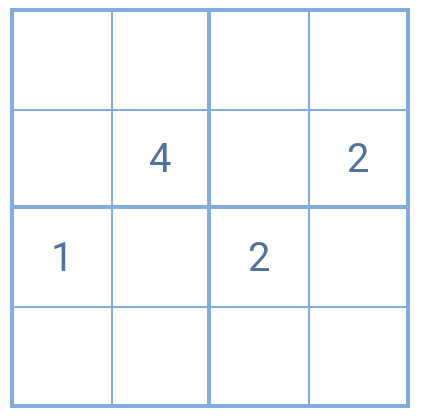
\includegraphics[width=.2\linewidth]{logic-based-classification/example_sudoku_board.png}
\end{center}

1. Extract the relevant information from an example. Here we extract the positions of the digits on the board.
These can be represented by the predicates:
\begin{verbatim}
    value(2, 2, 4). value(3, 1, 1). 
    value(2, 4, 2). value(3, 3, 2).
\end{verbatim}
where \verb_value_ stores row, column and digit information in that order.

2. Generate the example string. 
The example context will consist of information extracted in step 1, the inclusion of the true label, while the exclusion would contain all of the incorrect labels.
Finally, the penalty is computed from $\text{round} \left ( -\frac{K}{I} \ln \left ( \frac{\epsilon}{1 - \epsilon} \right ) \right )$.
If we set the values for constants $K, I,$ and $\epsilon$ to $1000, 100$ and $0.01$ and consider the binary version of the sudoku task, we get the following example:

\begin{verbatim}
#pos(id@46,
{ selected(valid) },
{ selected(invalid) },
{
 value(2, 2, 4). value(3, 1, 1). 
 value(2, 4, 2). value(3, 3, 2).
}).
\end{verbatim}

3. Generate the prior penalties.
Choosing the values for parameters $m_l$ is done through empirical evaluation, while $n_l$ is determined from a language bias.
The former is the number of rules of length $m_l$ that we expect in a final solution, while the latter is the total number of rules with length $l$ from the current language bias:

\begin{verbatim}
#modeh(selected(invalid)).

#modeb(row(var(cell), var(row))).
#modeb(value(var(cell), var(num))).

#maxv(4).
\end{verbatim}

Clearly we can have 2 rules of length 1 (head + each body), so $n_1$ is 2.
Also, $n_2 = 2$ since only the following rules exists:
\begin{verbatim}
selected(invalid) :- row(V3,V4); value(V1,V2).
selected(invalid) :- row(V1,V3); value(V1,V2).
\end{verbatim}
They need to be defined so that their types match, are unique, and are not trivially replaceable by another rule.
The last requirement means that we do not allow rules such as $selected(invalid) \; \text{:-} \; row(V1, V3), row(V2, V4)$ since row(1, 1) would make this rule true.

Setting empirically determined values $m_1 = m_2 = 1$, results in the following hypothesis penalties.
\begin{lstlisting}
penalty(P, custom) :- L = #count{X : in_head(X); X : in_body(X)}, pen(L, P).
pen(1, 0).
pen(2, 0).
pen(L, 100000000000) :- L = #count{X : in_head(X); X : in_body(X)}, 
    L >= 3.
\end{lstlisting}

The values for parameters $n_l$ are in practice approximated using $\binom{r}{l}$, the number of possible selections of l predicates from r \verb_#modeb_ definitions.
Note that this approximation is completely accurate when we only have constant \verb_#modeb_ declarations, which is the case for the concept bottleneck pipeline.

Further extensions to this system should make this value more accurate, but it did not hurt performance.

\end{example}


A simple, yet extremely beneficial, implemented performance optimisation is \textbf{example aggregation}. \\
When sampling $I$ values, track each outcome and its number of occurrences before generating the actual examples.
The tracking allows to replace $C$ identical examples of penalty $\text{round} \left ( -\frac{K}{I} \ln \left ( \frac{\epsilon}{1 - \epsilon} \right ) \right )$ with only one example of penalty $C * \text{round} \left ( -\frac{K}{I} \ln \left ( \frac{\epsilon}{1 - \epsilon} \right ) \right )$, reducing the overall FastLAS running time.

% \subsubsection{Search Space Counting}
% TODO: Finish Implementation

\section{Evaluation}

The evaluation is carried out on two tasks: 
\begin{enumerate}
    \item Sudoku grid validity
    \item MLB-V2E classification
\end{enumerate}

The former is a much simpler task which will evaluate whether the method does indeed work well, while the latter will consider the Prob-FF-NSL framework within the context of a concept bottleneck pipeline.

\subsection{Sudoku grid learning}
\label{sudoku-grid-learning}

This task aims to determine whether a sudoku grid with hand-written digits is valid, i.e. there are no repeated numbers in a block, row or column.
% INSERT FF-NSL DONE
It is the repeat of the task studied in \cite{RefWorks:RefID:71-cunnington2021ff-nsl:}.
There are two versions of it, 4x4 and 9x9 sudoku grid validity tasks.

The digit values are treated as concepts in this example, while their probabilities are obtained from a digit-predicting neural network.

Given that this task is simple to tackle for a logic-based learning system and a standard CNN, it is explored when different percentages of digit images are subject to a distribution shift.
The distribution shift, in this case, is a 90-degree image rotation.
It significantly impacts the overall task, reducing the accuracy of digit prediction from 99\% to 14\%.

We will compare our approach to three baselines: random forest, CNN-LSTM architecture and FF-NSL architecture. 
The latter similarly uses example penalties to give higher penalties to more likely examples, but Cunnington et al. \cite{RefWorks:RefID:71-cunnington2021ff-nsl:} selected the example penalties through empirical evaluation.
% INSERT reference to section with FF-NSL
It is explained in more detail in \ref{probabilistic-rule-learning}.
Moreover, the FF-NSL and Prob-FF-NSL are tested using the same digit predictor network.

The learned models are compared with the true and shifted test sets.
The former always presents the correct digit prediction to the framework, while the latter has the same proportion of digit images shifted as the Prob-FF-NSL/FF-NSL training set.

The results for the sudoku 4x4 task are shown in the figure \ref{sudoku4x4-results}.

\begin{figure}[h]
% INSERT reference FF-NSL DONE
\caption{A comparison of the sudoku 4x4 task performance with an increasing level of distribution shifts. Adapted from Cunnington et al. \cite{RefWorks:RefID:71-cunnington2021ff-nsl:}}
\centering
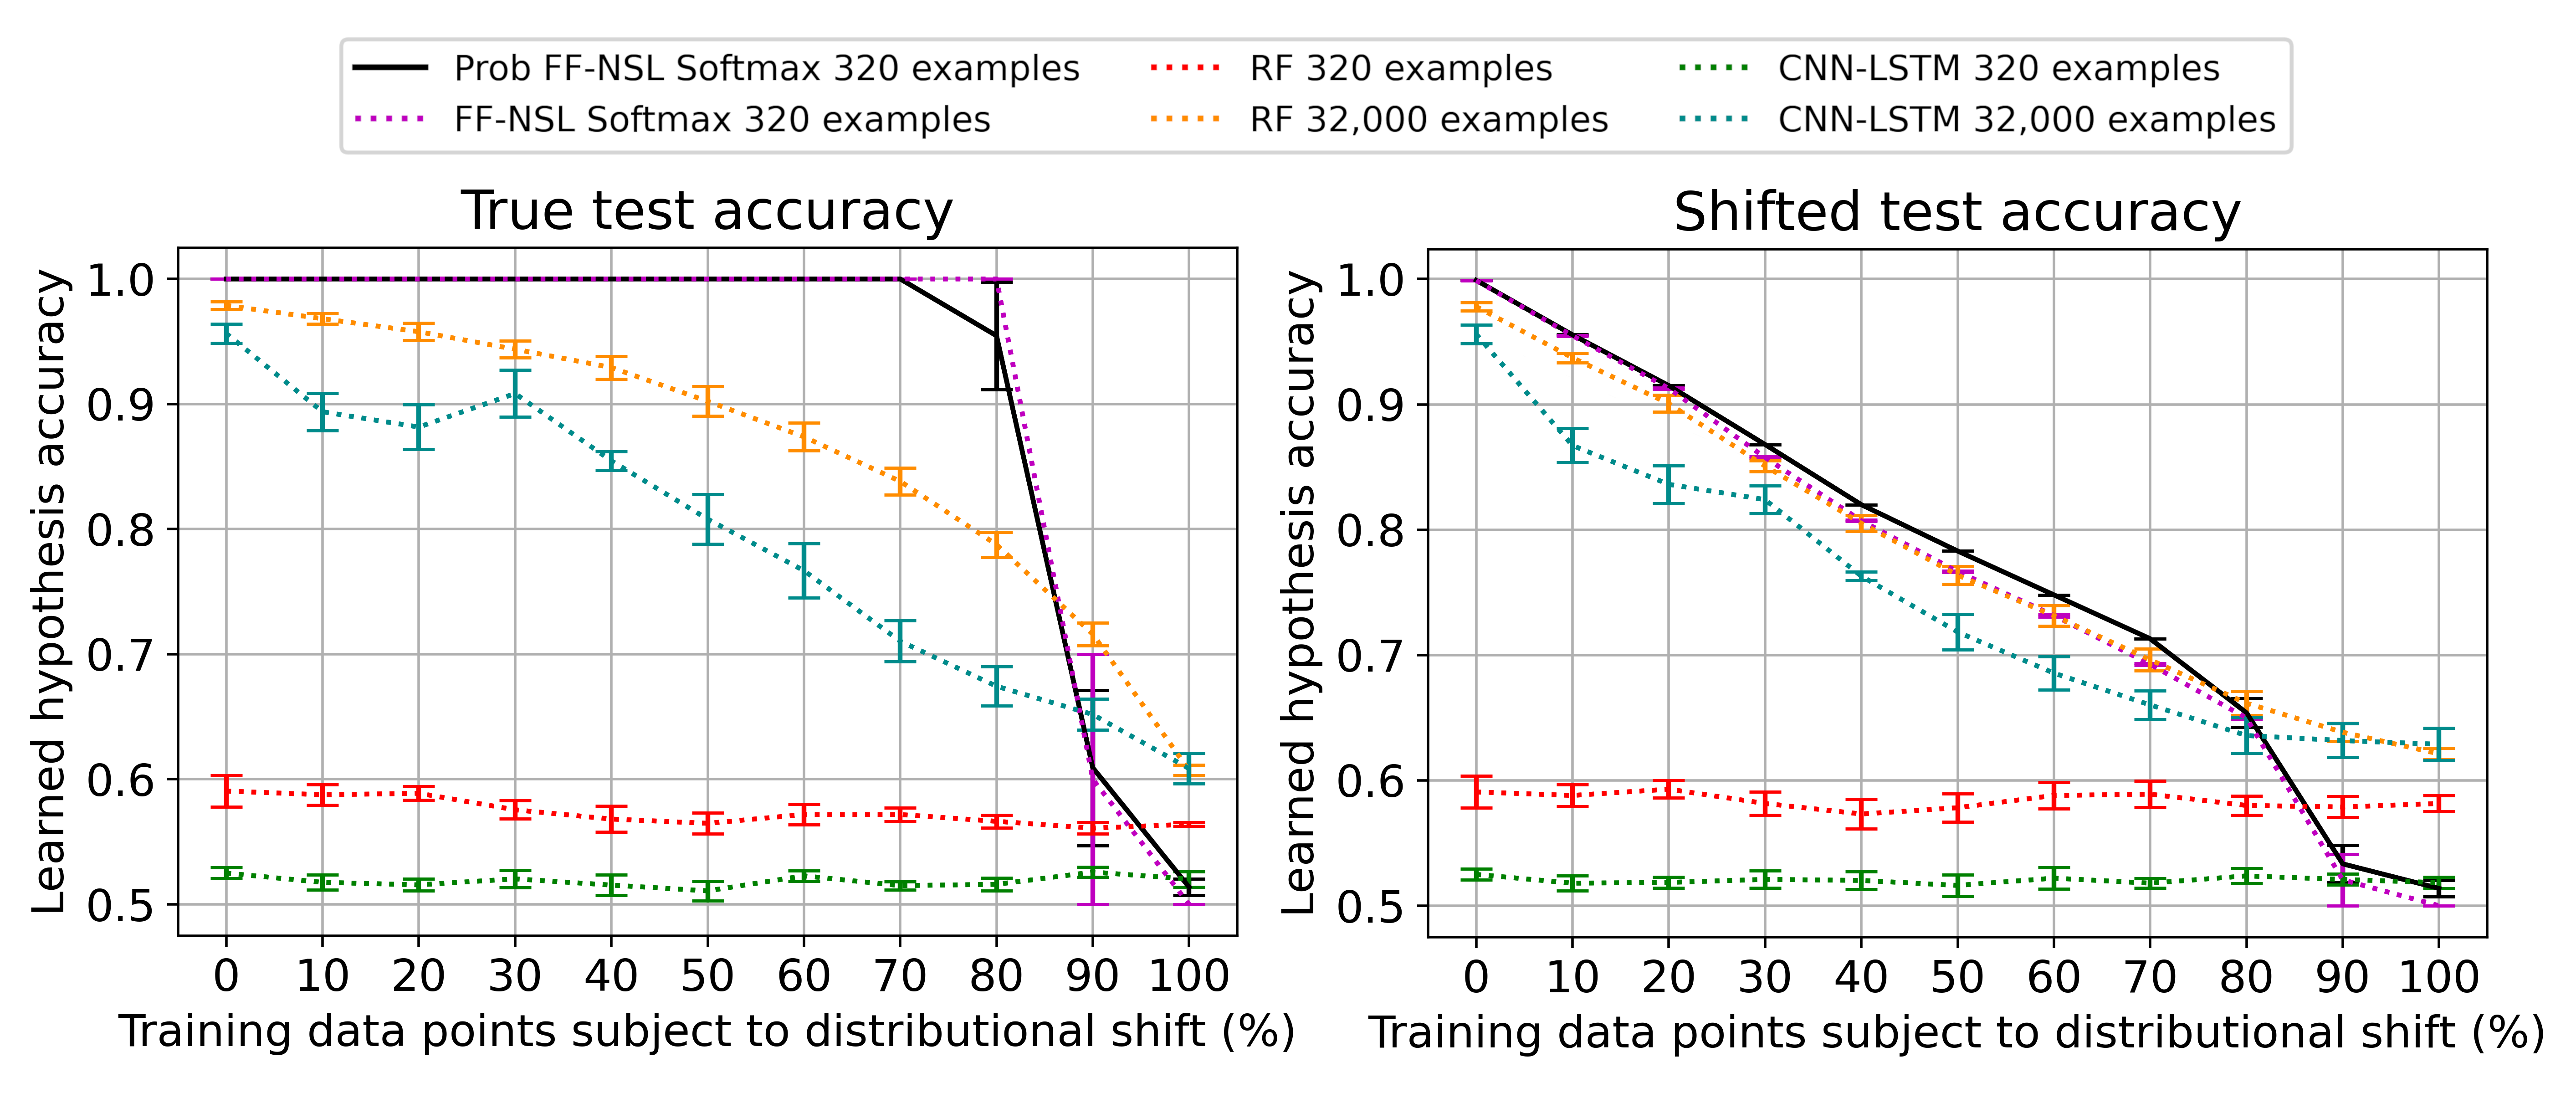
\includegraphics[width=\textwidth]{logic-based-classification/sudoku4x4.png}
\label{sudoku4x4-results}
\end{figure}

The results demonstrate that the Prob-FF-NSL and FF-NSL can learn the correct solution in spite of a high distribution shift.
They cover all of the true test examples even when 70\%/80\% of examples are subject to a distribution shift.
Both approaches have an almost identical performance dealing with a shifted test set.
On the other hand, the LSTM-CNN and the random forest fail to learn a correct solution even when given ten times more examples.
The models with more examples perform comparably to the FF-NSL approaches on a shifted test set.
With only 320 examples, they fail to learn a solution with their performance slightly above 0.5, which is a threshold that a random model would achieve.

The results for sudoku 9x9, presented in \ref{sudoku9x9-results}, show similar results.
\begin{figure}[h]
% INSERT reference FF-NSL DONE
\caption{A comparison of the sudoku 9x9 task performance with an increasing level of distribution shifts. Adapted from Cunnington et al. \cite{RefWorks:RefID:71-cunnington2021ff-nsl:}}
\centering
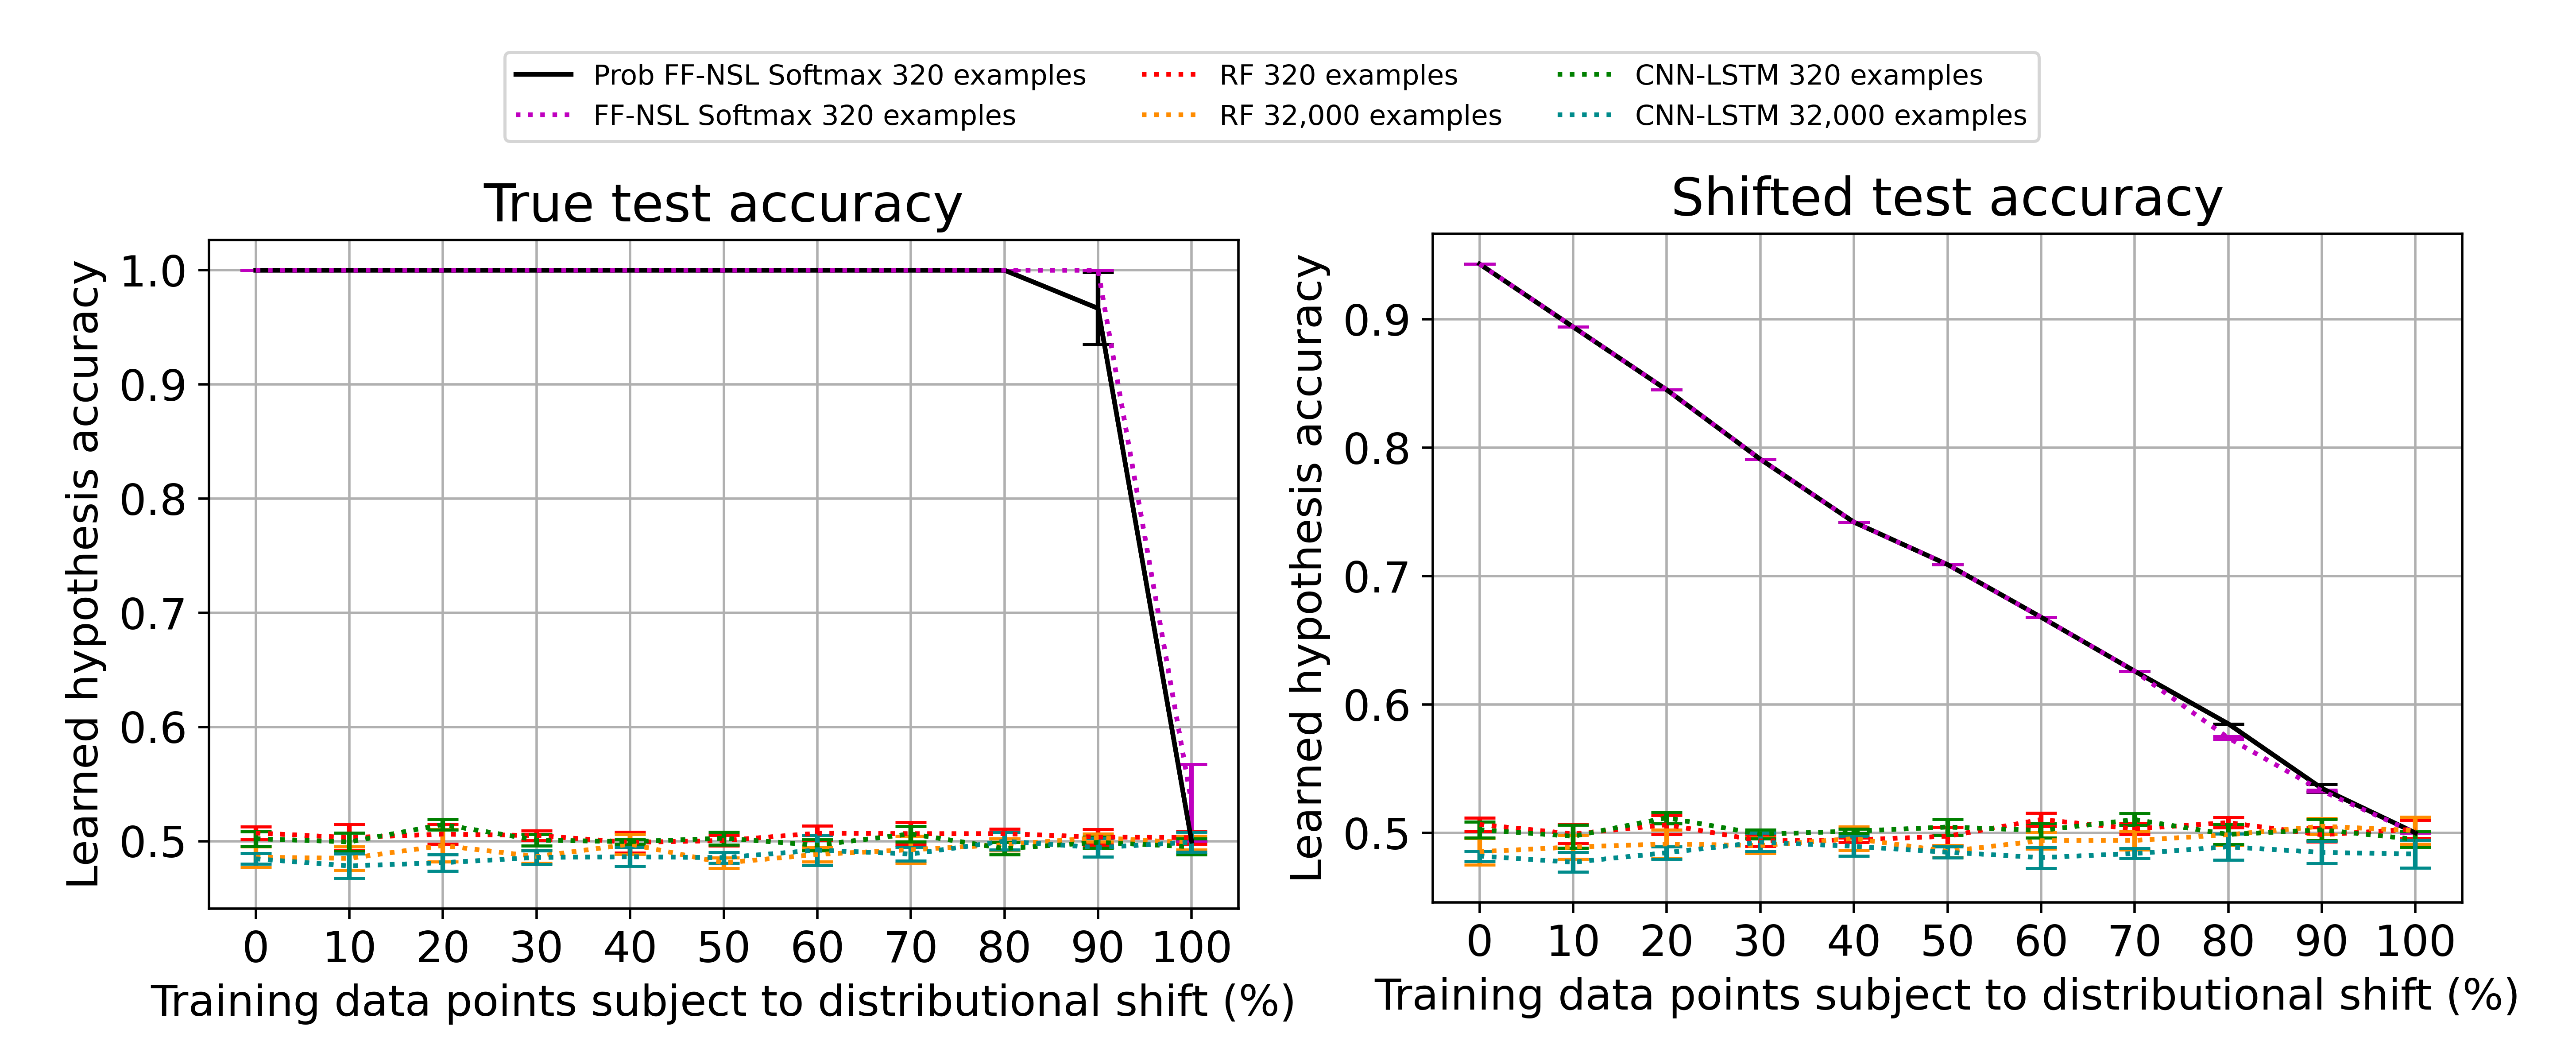
\includegraphics[width=\textwidth]{logic-based-classification/sudoku9x9.png}
\label{sudoku9x9-results}
\end{figure}

The main difference in performance is present for the random forest and CNN-LSTM baseline models, which failed to learn a good solution.

The model returned the following rules in all cases where the true test accuracy was 100\%:
\begin{lstlisting}
selected(invalid) :- neq(V0,V1), neq(V1,V0), value(V0,V2), value(V1,V2), row(V0,V3), row(V1,V3), cell(V0), cell(V1), num(V2), row(V3).
selected(invalid) :- block(V1,V0), block(V2,V0), neq(V1,V2), neq(V2,V1), value(V1,V3), value(V2,V3), block(V0), cell(V1), cell(V2), num(V3).
selected(invalid) :- neq(V0,V1), neq(V1,V0), col(V0,V2), col(V1,V2), value(V0,V3), value(V1,V3), cell(V0), cell(V1), col(V2), num(V3).
\end{lstlisting}
These rules are clearly correct as they outline that no row, block or column can have two of the same digits.


All in all, the Prob-FF-NSL performs well, having a perfect true test score in spite of 70\%/80\% of examples under a distribution shift for the sudoku problems.
However, it performs slightly worse than the FF-NSL method on this particular task. 
The advantage of the FF-NSL approach is that it assigns more importance to training examples that are not under the distribution shift.
But, the Prob-FF-NSL also accounts for the non-maximum predictions in its training, so the slight difference may only be down to the random seeds used when sampling.
Finally, the FF-NSL models performed much better than the others as they incorporated background knowledge.


\subsection{Concept Bottleneck Pipeline}

We also test the presented Prob-NSL framework within the context of a concept bottleneck model.
The architecture that the Prob-NSL model used for this task is presented in \ref{change-to-the-concept-bottleneck-architecture}.

As baselines, we compare the model to an end-to-end network and the concept bottleneck model with identical architectures.
The latter is the same model used for the concept prediction for the Prob-FF-NSL model.

Their results are summarised in the table below:

\begin{center}
\begin{tabular}{ |M{3cm}|M{3cm}|M{3cm}|  }
 \hline
 \multicolumn{3}{|c|}{Test Accuracy Comparison} \\
 \hline
 \hline
  End-to-end model&Concept bottleneck model & Prob-NSL concept bottleneck \\ 
 \hline
 0.687 $\pm$ 0.004 & 0.685 $\pm$ 0.005 & 0.650 $\pm$ 0.016 \\
 \hline
\end{tabular}
\end{center}

The Prob-NSL model greatly outperforms the other two with 33\% test higher test set accuracy.
The results could have been even higher if the concept bottleneck model could distinguish between the labels \emph{strike} and \emph{ball} well.
In some instances, the model predicts a \emph{strike} in every case where the true label was \emph{ball}.
When the model learns well enough to distinguish between the two, the accuracy jumps to values as high as 96\%.

A learned solution can be post-processed into the following form:
\begin{lstlisting}
conds(strike) :- concept("The batter fouled it.").
conds(strike) :- concept("The batter hit the ball into foul territory."), concept("The ball was."), concept("The batter did not swing.").
conds(strike) :- concept("The batter made contact."), concept("The batter missed."), concept("The umpire called it a ball.").
conds(strike) :- concept("The batter did not swing."), concept("The ball was hit.").
conds(strike) :- concept("It was a strike."), concept("The batter did not swing.").
conds(foul) :- concept("It was outside the strike zone."), concept("The batter hit a fly ball.").
conds(foul) :- concept("The batter hit the ball into foul territory."), concept("The umpire called it a ball.").
conds(foul) :- concept("The batter hit the ball for a foul ball."), concept("The batter did not swing.").
conds(foul) :- concept("The batter hit the ball into foul territory."), concept("The batter hit the ball.").
conds(out) :- concept("The batter hit a fly ball."), concept("It hit the ground.").
conds(out) :- concept("The batter hit the ball for a foul ball."), concept("It was caught.").
conds(play) :- concept("The batter hit the ball in the air.").
\end{lstlisting}

At test time, the solver returns the head of the first rule whose rule body is satisfied if reading the rules from top to bottom.
If none of these rules is matched, the \emph{ball} label is returned.
Such an interpretation allows for a clear link between the concepts and the final labels.

However, inspecting the solution shows that it does not always follow baseball logic precisely. For example, the concept \emph{the batter fouled it} should not result in a strike.
The most likely cause of this result is that the neural network does not learn concepts as intended but instead uses them as proxies to incorporate its features.
With this in mind, we attribute the difference in performance to the concept prediction architecture of the original models, which only has a single linear layer.


\section{Discussion}

The proposed logic-based classification method works well but fails to learn an interpretably correct solution for the concept bottleneck model. Some cases do not 
follow human logic.
To account for this issue, we should improve upon the concept prediction pipeline, which currently has a precision of 17.5\%.

In general, the performance of the logic-based classification method on its own could further be improved by, for example, incorporating the example importance into the choice of the parameters.
Moreover, the approach for choosing a prior may not be flexible enough for all possible applications.
Incorporating the configurable prior approach shown by Drozdov et al. \cite{RefWorks:RefID:67-drozdov2021online} would have a lot of benefit in some cases.

% TODO: Luke feedback -random forest -feature importance - how often a predicate gets used to make a prediction 